\documentclass[12pt,a4paper]{report}

\usepackage[utf8]{inputenc}
\usepackage[T1]{fontenc}
\usepackage[spanish,es-tabla]{babel}
\usepackage{lmodern}
\usepackage{graphicx}
\usepackage[a4paper,margin=2.4cm]{geometry}
\usepackage{amsmath,amssymb,amsthm}
\usepackage{booktabs}
\usepackage{array}
\usepackage{multirow}
\usepackage{makecell}
\usepackage{subcaption}
\usepackage{float}
\usepackage{enumitem}
\usepackage{tikz}
\usetikzlibrary{arrows.meta,positioning,fit,backgrounds,decorations.pathreplacing}
\usepackage{eurosym}
\usepackage[hidelinks]{hyperref}

\graphicspath{{../figures/}}

\renewcommand{\topfraction}{0.92}
\renewcommand{\bottomfraction}{0.9}
\renewcommand{\textfraction}{0.08}
\renewcommand{\floatpagefraction}{0.82}
\setcounter{topnumber}{3}
\setcounter{totalnumber}{4}

\theoremstyle{definition}
\newtheorem{definicion}{Definición}
\newtheorem{teorema}{Teorema}

\setlist[itemize]{itemsep=2pt,topsep=3pt,parsep=0pt}

\AtBeginDocument{\def\%{\char37\relax}\shorthandoff{<>}}

\begin{document}

\chapter{Metodología}

El propósito de este capítulo es reunir los fundamentos que sostienen el
caso práctico. La metodología se organiza en tres bloques encadenados. El \textbf{bloque de text
mining} convierte cada texto en datos estructurados sobre los que un algoritmo puede calcular. El
\textbf{bloque de procesamiento de datos} construye, a partir de esa representación, las variables con
poder predictivo y reduce su dimensión. El \textbf{bloque de modelización analítica} ajusta los
clasificadores sobre esas variables, los valida y compara con distintas métricas. La
Figura~\ref{fig:bloques} resume el flujo. Cada bloque se detalla a continuación en su forma general.
Su aplicación concreta, con los datos, las variables y las cifras del problema, se reserva para el
capítulo siguiente.

\begin{figure}[H]
\centering
\begin{tikzpicture}[
  bloque/.style={rectangle, rounded corners, draw, align=center, minimum height=1.35cm,
                 text width=3.3cm, font=\small, fill=blue!6}]
\node[bloque](tm){Text mining};
\node[bloque, right=1.1cm of tm](pd){Procesamiento\\de datos};
\node[bloque, right=1.1cm of pd](ma){Modelización\\analítica};
\draw[-{Stealth}, thick](tm)--(pd);
\draw[-{Stealth}, thick](pd)--(ma);
\end{tikzpicture}
\caption{Los tres bloques de la metodología y el orden en que se aplican.}
\label{fig:bloques}
\end{figure}

% ###########################################################################
\section{Bloque de text mining}
\label{sec:textmining}

El dato de partida es texto, pero los clasificadores que usaremos operan sobre vectores de números
reales. La minería de textos (\emph{text mining}) \cite{aggarwal2012textmining} es el conjunto de
técnicas que salva esa distancia: transforma un texto en una representación numérica sobre la que un
modelo pueda calcular. Este bloque recorre las piezas de esa transformación en el orden en que se
aplican, de las unidades mínimas del texto hasta la matriz de números que las resume.

\medskip
\noindent\textbf{Tokenización.} El primer paso divide el texto en unidades mínimas llamadas
\emph{tokens}, normalmente las palabras. Una tokenización simple extrae las secuencias alfanuméricas
maximales y descarta los signos de puntuación, de modo que la frase queda reducida a una lista de
palabras. La frase ``El hotel tiene WiFi gratis.'' produce los cinco tokens
$\langle$el, hotel, tiene, WiFi, gratis$\rangle$. Sobre esa lista actúan los pasos siguientes.

\medskip
\noindent\textbf{Normalización.} Distintas escrituras de una misma palabra deben tratarse como una
sola. La normalización reduce esas variantes a una forma común, y agrupa varias operaciones
independientes.

\begin{itemize}
\item \textbf{Paso a minúsculas.} Convierte todo el texto a minúsculas para que ``WiFi'' y ``wifi'' no
cuenten como términos distintos.
\item \textbf{Eliminación de \emph{stopwords}.} Descarta las palabras vacías, aquellas muy frecuentes
que apenas aportan significado (artículos, preposiciones, conjunciones como ``de'', ``el'', ``y''). 
\item \textbf{\emph{Stemming}.} Recorta cada palabra a su raíz aplicando reglas de sufijos, sin
consultar un diccionario. Así ``jugando'', ``jugador'' y ``jugaba'' se reducen todas a ``jug''. Es
rápido, pero la raíz que produce no siempre es una palabra real.
\item \textbf{Lematización.} Lleva cada palabra a su forma de diccionario (su \emph{lema}) usando su
categoría gramatical: ``jugando'' pasa a ``jugar'', ``mejores'' a ``bueno''. Es más precisa que el
\emph{stemming} y más costosa, porque necesita analizar la palabra en su contexto.
\end{itemize}

\medskip
\noindent\textbf{Bolsa de palabras.} La representación más básica de un texto es la \emph{bolsa de
palabras}~\cite{harris1954distributional}. Se fija un vocabulario de $V$ términos, uno por cada palabra
distinta de la colección, y cada texto se convierte en una fila de una matriz de documentos por
tokens: la celda correspondiente cuenta cuántas veces aparece ese término en ese documento, sin atender
al orden en que aparecen. Con los documentos ``free wifi hotel'', ``wifi hotel breakfast'' y ``cheap
hotel'', el vocabulario tiene cinco términos y la matriz de frecuencias es:

\begin{center}
\begin{tabular}{lccccc}
\toprule
 & free & wifi & hotel & breakfast & cheap \\
\midrule
$d_1$: free wifi hotel      & 1 & 1 & 1 & 0 & 0 \\
$d_2$: wifi hotel breakfast & 0 & 1 & 1 & 1 & 0 \\
$d_3$: cheap hotel          & 0 & 0 & 1 & 0 & 1 \\
\bottomrule
\end{tabular}
\end{center}

\medskip
\noindent\textbf{$n$-gramas.} La bolsa de palabras pierde el orden, y con él parte del significado:
``no funciona'' dice lo contrario que ``funciona''. Los \emph{$n$-gramas} recuperan algo de ese orden
tomando como unidad grupos de $n$ tokens consecutivos en vez de palabras sueltas. Un unigrama es una
palabra aislada; un bigrama, dos seguidas (``wifi gratis''); un trigrama, tres. Retener bigramas
captura combinaciones que la palabra aislada no distingue, pero cada nivel de $n$-grama multiplica el
tamaño del vocabulario, así que en la práctica el $n$ se mantiene bajo.

% ###########################################################################
\section{Bloque de procesamiento de datos}
\label{sec:procesamiento}

Con el texto ya troceado, este bloque construye las variables numéricas que alimentan al modelo. La
tarea es doble: pasar de simples conteos de palabras a pesos que reflejen lo informativa que es cada
una, y reducir la enorme dimensión de esa representación a un espacio manejable que conserve el
significado.

\medskip
\noindent\textbf{Ponderación TF-IDF.} La matriz de frecuencias da el mismo peso a una palabra vacía muy
repetida que a un término informativo raro. El esquema \textbf{TF-IDF} (\emph{term frequency--inverse
document frequency}) corrige ese sesgo ponderando cada término por su rareza en la colección
\cite{salton1988tfidf}: pesa mucho lo específico y poco lo frecuente. Sea una colección de $N$
documentos; para un término $t$, denotamos por $\mathrm{tf}(t,d)$ el número de veces que $t$ aparece en
el documento $d$ y por $\mathrm{df}(t)$ el número de documentos que contienen $t$. El peso de $t$ en
$d$ es el producto de dos factores,
\begin{equation}
w_{t,d} \;=\; \underbrace{\mathrm{tf}(t,d)}_{\text{frecuencia en el documento}}\;\cdot\;
\underbrace{\log\frac{N}{\mathrm{df}(t)}}_{\text{rareza en la colección}}.
\label{eq:tfidf}
\end{equation}
El primer factor, la frecuencia de término, sube con las veces que $t$ aparece en el documento; el
segundo, la frecuencia inversa de documento, lo penaliza si además aparece en muchos documentos. La
intuición del segundo factor es una medida de sorpresa: un término presente en casi todos los
documentos tiene $\mathrm{df}(t)\approx N$, su logaritmo tiende a cero y su peso se anula, porque su
presencia no aporta información; uno raro tiene $\mathrm{df}(t)$ pequeño y su logaritmo crece.

Sobre el ejemplo de la bolsa de palabras, con $N=3$ y tomando logaritmo natural, el factor de rareza
de cada término es:
\begin{center}
\begin{tabular}{lcc}
\toprule
término & $\mathrm{df}(t)$ & $\ln(N/\mathrm{df}(t))$ \\
\midrule
hotel                  & 3 & $\ln(3/3)=0$ \\
wifi                   & 2 & $\ln(3/2)\approx 0{,}41$ \\
free, breakfast, cheap & 1 & $\ln(3/1)\approx 1{,}10$ \\
\bottomrule
\end{tabular}
\end{center}
La palabra ``hotel'', presente en los tres documentos, recibe peso cero: es común y no discrimina entre
documentos. Las que solo aparecen en uno reciben el peso máximo, porque son las que lo caracterizan
frente al resto. Así, la fila de $d_1$ deja de ser $(1,1,1,0,0)$ y pasa a
$(1{,}10,\,0{,}41,\,0,\,0,\,0)$: el peso se concentra en ``free'' y ``hotel'' se anula.

\medskip
\noindent\textbf{Vectores TF-IDF.} Aplicada a toda la colección, la ponderación convierte cada
documento en un \emph{vector TF-IDF} de $\mathbb{R}^V$, una fila con un peso por cada término del
vocabulario. Apiladas, esas filas forman la matriz TF-IDF $M\in\mathbb{R}^{N\times V}$, con un
documento por fila y un término por columna. Es la representación numérica del texto sobre la que
trabajan tanto las medidas de parecido entre documentos como los modelos.

% ###########################################################################
\section{Bloque de modelización analítica}
\label{sec:modelizacion}

Con las variables ya construidas, este bloque las convierte en un clasificador. Un modelo de
aprendizaje automático es un programa que aprende a reconocer patrones a partir de
ejemplos~\cite{mitchell1997ml}: se le muestra un conjunto de datos ya resueltos y ajusta sus parámetros
para reproducirlos; una vez ajustado, puede predecir sobre datos nuevos, no empleados en el entrenamiento. Según lo que se
conozca de los ejemplos se distinguen dos grandes tipos. En el \textbf{aprendizaje supervisado} los
ejemplos vienen etiquetados con la respuesta correcta y el modelo aprende a predecirla; es el que
usamos aquí. En el \textbf{aprendizaje no supervisado} no hay etiqueta y el modelo agrupa los datos por
semejanza; queda fuera de este trabajo.

Cada ejemplo se describe por unas medidas y lleva asociada una respuesta: las medidas son las
\emph{características} y la respuesta es la \emph{clase}. Una característica es cada magnitud que se mide
de un ejemplo, y el vector de características $x=(x_1,\dots,x_d)\in\mathbb{R}^d$ las reúne todas; la
clase $y$ es la respuesta asociada, y en clasificación binaria toma dos valores, $y\in\{0,1\}$. Con $n$
ejemplos, la base de datos es el conjunto $\{(x_i,y_i)\}_{i=1}^{n}$, que apilado por filas forma la
matriz de características $X\in\mathbb{R}^{n\times d}$ y el vector de etiquetas $y\in\{0,1\}^n$. El
objetivo es estimar una función $f\colon\mathbb{R}^d\to\{0,1\}$ que, dado un $x$ nuevo, prediga su
clase. Lo que importa es que \textbf{generalice}: que acierte sobre datos nuevos, no solo sobre los que
aprendió. El obstáculo es el \textbf{sobreajuste}, un modelo con demasiada capacidad memoriza el ruido
del entrenamiento y falla fuera de él, y se entiende por el compromiso \textbf{sesgo--varianza}
\cite{geman1992biasvariance}: un modelo demasiado rígido tiene sesgo alto y no captura la estructura de
los datos, uno demasiado flexible tiene varianza alta y se pliega a cada fluctuación; el buen
rendimiento está en el punto intermedio. Ningún modelo es el mejor para todo problema
\cite{wolpert1996nfl}, por lo que en la práctica se entrenan varios y se compara su rendimiento.

Ese proceso sigue un flujo ordenado de fases. Existen metodologías que lo estructuran. En nuestro caso adoptamos
\textbf{SEMMA} \cite{azevedo2008semma}, propuesta por el SAS Institute e implementada en la herramienta
SAS Enterprise Miner, que organiza la minería de datos en cinco fases:

\begin{itemize}
\item \textbf{Exploración} (\emph{Explore}): describir los datos, sus distribuciones, la prevalencia de
cada clase y las relaciones entre variables.
\item \textbf{Muestreo} (\emph{Sample}): fijar los conjuntos de entrenamiento, validación y test, y
equilibrar las clases si el reparto es muy desigual.
\item \textbf{Modificación} (\emph{Modify}): depurar y preparar las variables (valores ausentes,
atípicos) y seleccionar las informativas.
\item \textbf{Modelización} (\emph{Model}): ajustar los modelos y sus hiperparámetros.
\item \textbf{Valoración} (\emph{Assess}): medir el rendimiento de los modelos ajustados con métricas.
\end{itemize}

\begin{figure}[H]
\centering
\resizebox{\textwidth}{!}{%
\begin{tikzpicture}[
  every node/.style={font=\footnotesize},
  fase/.style={rectangle, rounded corners, draw=green!45!black, thick, fill=green!12,
               align=center, minimum height=0.9cm, text width=2.2cm, inner sep=3pt},
  lbl/.style={font=\itshape},
  crisp/.style={font=\itshape, align=center},
  link/.style={-{Stealth[length=4pt]}, draw=black!55}]

\node[fase] (mu)  at (4.1,6)   {Muestreo (sí/no)};
\node[fase] (vis) at (2.4,4.5) {Visualización de datos};
\node[fase] (clu) at (5.8,4.5) {Clustering (agrupación)};
\node[fase] (sel) at (2.4,3)   {Selección de variables};
\node[fase] (tra) at (5.8,3)   {Transformación de datos};
\node[fase] (arb) at (0.6,1.5) {Árbol de decisión};
\node[fase] (rl)  at (3.05,1.5){Regresión logística};
\node[fase] (rn)  at (5.5,1.5) {Redes neuronales};
\node[fase] (otr) at (7.95,1.5){Otros modelos};
\node[fase] (val) at (3.05,0)  {Valoración de modelos};

\node[lbl] at (-1.7,6)   {SAMPLE};
\node[lbl] at (-1.7,4.5) {EXPLORE};
\node[lbl] at (-1.7,3)   {MODIFY};
\node[lbl] at (-1.7,1.5) {MODEL};
\node[lbl] at (-1.7,0)   {ASSESS};

\draw[link] (mu)--(vis); \draw[link] (mu)--(clu);
\draw[link] (vis)--(sel); \draw[link] (clu)--(tra);
\draw[link] (sel)--(arb); \draw[link] (sel)--(rl);
\draw[link] (tra)--(rn);  \draw[link] (tra)--(otr);
\draw[link] (arb)--(val); \draw[link] (rl)--(val);
\draw[link] (rn)--(val);  \draw[link] (otr)--(val);

\draw[decorate,decoration={brace,amplitude=5pt}] (9.35,6.5)--(9.35,4);
\node[crisp] at (11,5.25) {DATA\\UNDERSTANDING};
\draw[decorate,decoration={brace,amplitude=5pt}] (9.35,3.5)--(9.35,2.5);
\node[crisp] at (11,3) {DATA\\PREPARATION};
\draw[decorate,decoration={brace,amplitude=5pt}] (9.35,2)--(9.35,1);
\node[crisp] at (11,1.5) {MODELING};
\draw[decorate,decoration={brace,amplitude=5pt}] (9.35,0.5)--(9.35,-0.5);
\node[crisp] at (11,0) {EVALUATION};
\end{tikzpicture}}
\caption{Esquema general de la organización de la minería de datos según SEMMA}
\label{fig:semma}
\end{figure}

\noindent Las cinco fases se desarrollan a continuación.

\subsection{Análisis exploratorio}

Antes de modelar es necesario entender los datos. El \textbf{análisis descriptivo} caracteriza cada variable y
la etiqueta: su distribución, su rango, sus valores atípicos y las relaciones que guardan entre sí y
con la clase. De este análisis salen las decisiones de las fases siguientes y afloran los problemas que
condicionan el resto del trabajo. Los descriptivos se presentan de dos formas complementarias, y la
elección depende de si interesa el resumen exacto o la forma de la distribución.

\medskip
\noindent\textbf{Tablas.} Resumen cada variable con estadísticos numéricos: su media, su desviación
típica, su mínimo y su máximo, y los cuartiles que marcan cómo se reparten los valores. Son la forma
compacta y exacta de leer una variable, y sirven también para contar las categorías de una variable
discreta.

\medskip
\noindent\textbf{Gráficos.} Muestran la forma de la distribución, que una tabla de estadísticos no deja
ver. Distinguimos dos usos:
\begin{itemize}
\item \textbf{Histograma univariante.} Reparte los valores de una variable en intervalos y dibuja una
barra por intervalo con la frecuencia de cada uno. Permite ver dónde se concentran los
datos, si la distribución es simétrica o sesgada, y si hay valores alejados del resto.
\item \textbf{Histograma cruzado con la clase.} Superpone, sobre los mismos intervalos, la distribución
de la variable en cada clase (aquí, respuestas limpias frente a alucinadas). Cuando las dos
distribuciones se separan, la variable discrimina y es candidata a predictor útil; cuando se solapan
por completo, la variable apenas distingue las clases.
\end{itemize}

\medskip
\noindent\textbf{Prevalencia y desbalance.} El problema más determinante que revela la exploración en
clasificación es el \textbf{desbalance} entre clases. La \emph{prevalencia} de una clase es la fracción
de ejemplos que le pertenecen; cuando una clase es mucho menos frecuente que la otra, el aprendizaje se
sesga hacia la mayoritaria, y un modelo que se limite a predecirla siempre acierta en apariencia sin
detectar un solo caso de la minoritaria. Si una clase supone el $90\,\%$ de los ejemplos, predecir
siempre la mayoritaria alcanza un $90\,\%$ de aciertos sin ninguna utilidad. Reconocer el desbalance a tiempo
orienta las tres decisiones posteriores: el muestreo con que se equilibra la base, el umbral con que se
decide y las métricas con que se juzga.

\subsection{Muestreo}

La fase de \textbf{muestreo} decide con qué datos se entrena y se evalúa el modelo. Comprende tres
cuestiones: si conviene trabajar con una muestra, cómo repartir los datos y cómo tratar el desbalance
entre clases.

\medskip
\noindent\textbf{Tomar una muestra.} Cuando la base es demasiado grande para ajustar los modelos en un
tiempo razonable, se trabaja con una muestra aleatoria representativa en lugar de con todos los datos,
sacrificando algo de información a cambio de un coste asumible.

\medskip
\noindent\textbf{Partición de los datos.} Para estimar el rendimiento sobre datos no vistos, los datos
se reparten en subconjuntos disjuntos:
\begin{itemize}
\item \textbf{Entrenamiento:} el modelo ajusta sobre él sus parámetros.
\item \textbf{Validación:} sirve para elegir los hiperparámetros sin contaminar la estimación final.
\item \textbf{Test:} se reserva hasta el final y se usa una sola vez para medir el rendimiento.
\end{itemize}
Cuando los datos escasean, apartar un bloque fijo de validación desperdicia ejemplos; en su lugar se
recurre a la validación cruzada que describiremos en la modelización, que rota el papel de validación
entre varias particiones del entrenamiento. En ese caso basta con separar entrenamiento y test.

\medskip
\noindent\textbf{Balanceo de clases.} Cuando el reparto de clases es muy desigual, conviene corregirlo
antes de entrenar. El \textbf{remuestreo} reequilibra la base de entrenamiento antes de ajustar el
modelo, de tres maneras:
\begin{itemize}
\item \textbf{Sobremuestreo} (\emph{oversampling}): añade ejemplos de la clase minoritaria hasta
igualar a la mayoritaria. En su forma más simple los duplica al azar, con el riesgo de que el modelo
memorice esos ejemplos repetidos.
\item \textbf{SMOTE} (\emph{Synthetic Minority Over-sampling Technique}): en lugar de duplicar, crea
ejemplos \emph{sintéticos} de la clase minoritaria interpolando entre cada ejemplo y sus vecinos más
cercanos, con lo que rellena la frontera sin repetir puntos \cite{chawla2002smote}.
\item \textbf{Submuestreo} (\emph{undersampling}): descarta ejemplos de la clase mayoritaria hasta
igualar a la minoritaria. Equilibra sin inventar datos, pero desperdicia información.
\end{itemize}
El remuestreo no es la única palanca frente al desbalance: ponderar las clases en la función de pérdida
(penalizar más los errores sobre la minoritaria) o ajustar el umbral de decisión consiguen un efecto
parecido sin modificar los datos.

\subsection{Manipulación de datos}

La fase de \textbf{modificación} prepara las variables antes de modelar. Depura los datos, corrigiendo
los valores ausentes y los atípicos, y reduce la dimensión quedándose con las variables informativas.
La construcción de las variables a partir del texto, la ingeniería de características, se describe en el
capítulo práctico; aquí tratamos la teoría de la depuración y la selección.

\medskip
\noindent\textbf{Valores ausentes.} Un valor ausente (\emph{missing}) es una casilla sin dato: la
variable no se midió, no se registró o no aplica a ese ejemplo. Importan porque muchos modelos no
admiten valores ausentes, y porque la razón de la ausencia puede sesgar el análisis. Se distinguen tres
mecanismos según de qué dependa que un dato falte \cite{little2019missing}:
\begin{itemize}
\item \textbf{Ausentes completamente al azar} (MCAR): la ausencia no guarda relación con ningún valor,
observado o no. Se pueden ignorar sin sesgo.
\item \textbf{Ausentes al azar} (MAR): la ausencia depende de otras variables observadas, pero no del
valor que falta. Se pueden imputar a partir de las variables conocidas.
\item \textbf{Ausentes no al azar} (MNAR): la ausencia depende del propio valor que falta. Son los más
problemáticos, porque ignorarlos introduce sesgo.
\end{itemize}
Ante un valor ausente caben dos vías: descartar el ejemplo, lo que desperdicia datos, o
\emph{imputarlo}, es decir, rellenarlo con un valor plausible. La imputación más simple sustituye el hueco
por la media o la mediana de la variable; otras estiman el valor faltante a partir de las demás
variables del ejemplo.

\medskip
\noindent\textbf{Valores atípicos.} Un valor atípico (\emph{outlier}) es una observación que se aparta
mucho del grueso de los datos, ya por un error de medida, ya por un caso extremo real. Se detectan por
reglas sobre la dispersión: un criterio habitual marca como atípico todo valor que caiga fuera del
rango $[Q_1 - 1{,}5\,\mathrm{RIC},\; Q_3 + 1{,}5\,\mathrm{RIC}]$, donde $Q_1$ y $Q_3$ son el primer y
tercer cuartil y $\mathrm{RIC}=Q_3-Q_1$ el rango intercuartílico \cite{tukey1977eda}. Los atípicos afectan sobre todo a
los modelos que dependen de distancias o de sumas de cuadrados, la regresión lineal y logística o el
$k$ vecinos más cercanos, donde un solo punto extremo puede sesgar el ajuste; los modelos basados en
árboles, que parten por umbrales, son mucho más robustos frente a ellos. Detectado un atípico, se
corrige si es un error, se acota a un valor límite (\emph{winsorización}) o se mantiene sin cambios cuando es
un caso real informativo.

\medskip
\noindent\textbf{Selección de variables.} Con muchas variables conviene conservar las informativas y
descartar las redundantes, tanto para mejorar el modelo como para entenderlo \cite{guyon2003selection}.
Los métodos se agrupan en tres familias:
\begin{itemize}
\item \textbf{Filtro.} Puntúan cada variable por una medida estadística de su relación con la etiqueta,
al margen del modelo. Son rápidos, pero ignoran las interacciones y la redundancia entre variables, así
que pueden quedarse con dos variables casi idénticas.
\item \textbf{Envolventes} (\emph{wrapper}). Usan el propio modelo como juez: prueban subconjuntos de
variables y seleccionan el que mejor valida. Capturan interacciones, a mayor coste.
\item \textbf{Embebidos.} Seleccionan durante el propio ajuste del modelo, sin una fase aparte. La
regularización L1 de la regresión logística, que lleva a cero los coeficientes de las variables
irrelevantes, es un ejemplo.
\end{itemize}
La \textbf{eliminación recursiva de características} (RFE) es un método envolvente muy usado
\cite{guyon2002rfe}: entrena con todas las variables, elimina la menos importante, reentrena y repite,
lo que produce un orden de importancia. El número final de variables se fija por el \emph{método del
codo}: se representa el rendimiento frente al número de variables y se corta en el punto a partir del
cual añadir más ya no aporta, donde la curva se dobla.

\subsection{Modelización}

Entrenar un clasificador es ajustar sus \emph{parámetros} para que reproduzca las etiquetas del
entrenamiento, minimizando una función de pérdida. Los modelos concretos se desarrollan más abajo;
queda antes un paso común a todos: fijar sus \emph{hiperparámetros}, las opciones que no se aprenden de
los datos (la profundidad de un árbol, el número de vecinos) y que hay que decidir de antemano.

\medskip
\noindent\textbf{Validación cruzada.} Medir el rendimiento sobre los mismos datos con que se entrena
infla el resultado, porque el modelo ya los conoce. Reservar una parte para test lo evita, pero
entonces el resultado depende de qué ejemplos quedaron en esa partición. La \textbf{validación cruzada}
de $k$ iteraciones elimina esa dependencia~\cite{stone1974crossval}: parte el entrenamiento en $k$
bloques, entrena con $k-1$ y valida con el restante, y repite rotando el bloque de validación
(Figura~\ref{fig:groupkfold}); el rendimiento final es el promedio de las $k$ rondas, que ya no depende
de una partición concreta.

Esta partición debe respetar la estructura de los datos. Cuando varios ejemplos comparten una misma
unidad, aquí un mismo documento fuente del que proceden varias respuestas, esa unidad tiene que caer
entera en un solo bloque. Si no, el modelo encuentra en validación una respuesta casi idéntica a otra vista
en entrenamiento y el resultado se infla por esa filtración. La variante que lo garantiza es el
\textbf{GroupKFold}, que agrupa por la unidad e impide que un documento aparezca a la vez en
entrenamiento y validación.

\begin{figure}[H]
\centering
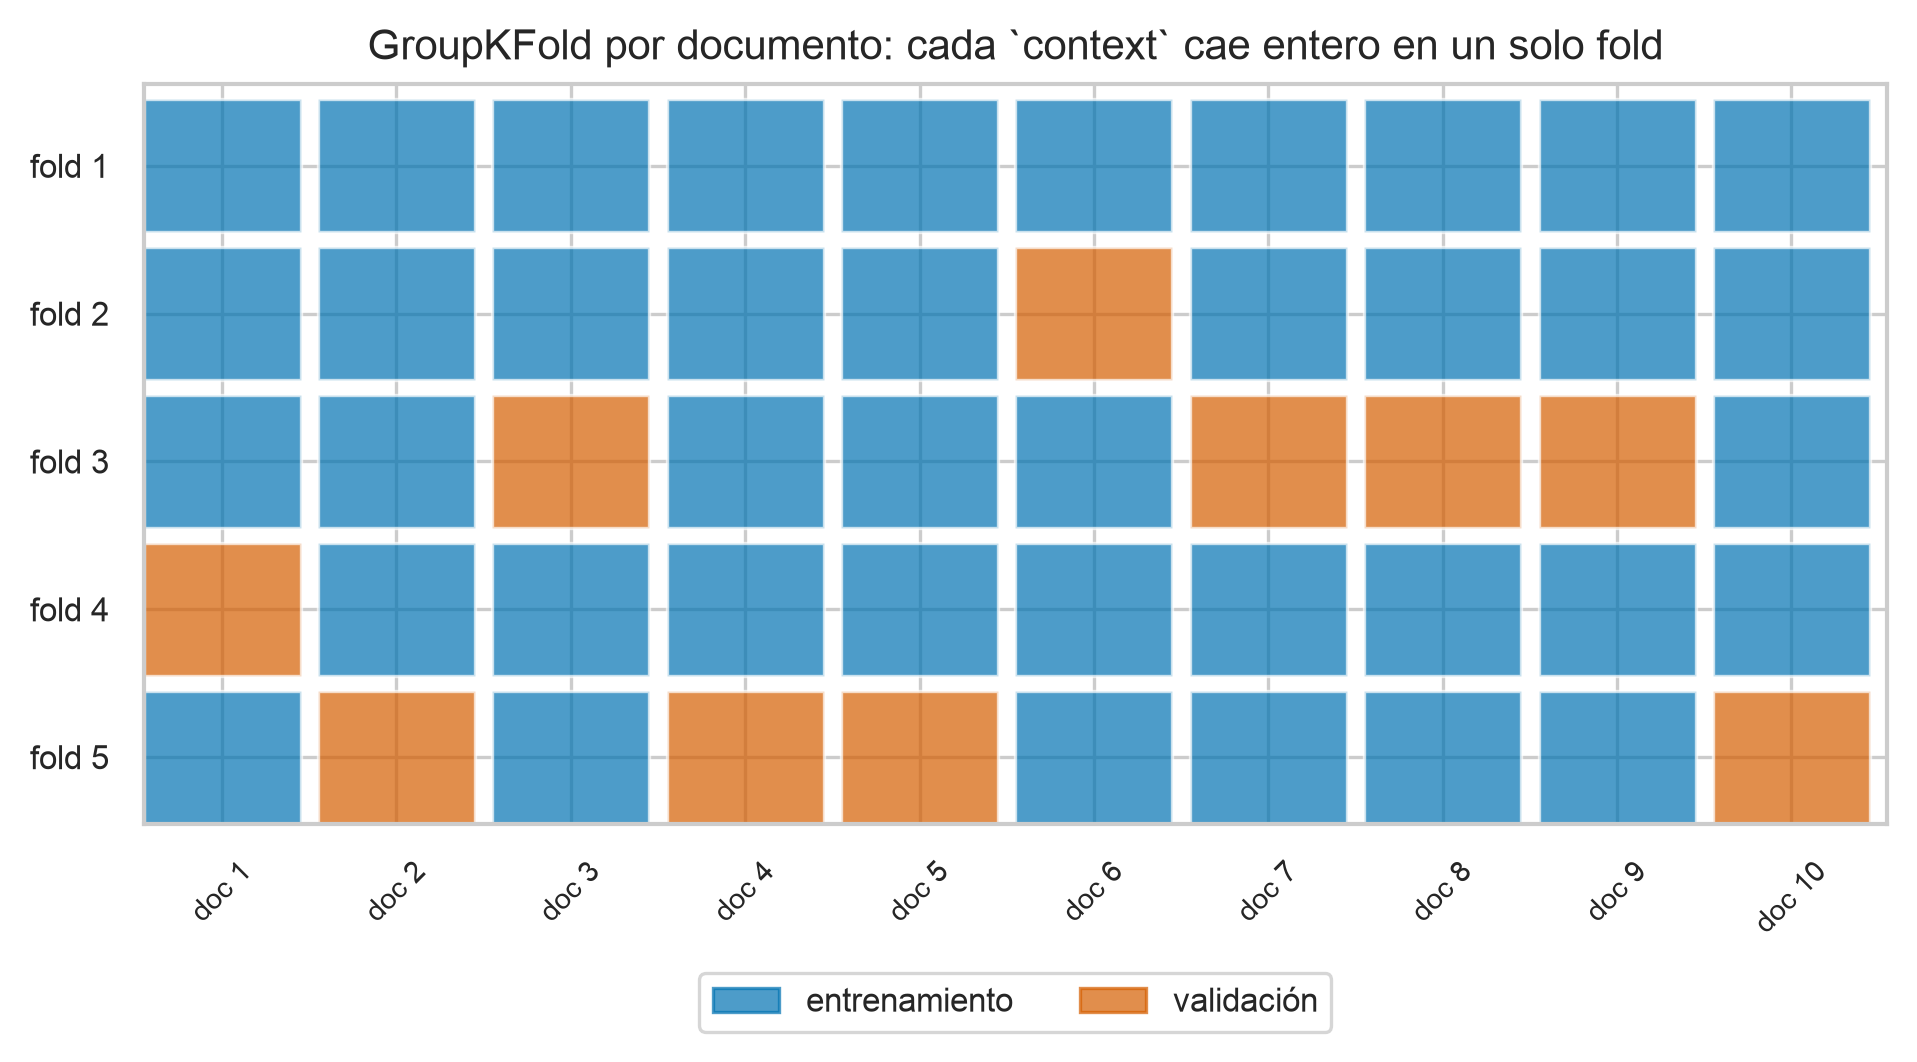
\includegraphics[width=0.62\textwidth]{concept_groupkfold}
\caption{GroupKFold por documento: cada fuente cae entera en un único bloque, de modo que ninguna
aparece a la vez en entrenamiento (azul) y validación (naranja).}
\label{fig:groupkfold}
\end{figure}

\medskip
\noindent\textbf{Búsqueda en rejilla.} Casi todos los modelos tienen hiperparámetros, y distintas
combinaciones dan resultados distintos: no es lo mismo tomar los $3$ vecinos más cercanos con distancia
euclídea que los $11$ con distancia de Manhattan. La \textbf{búsqueda en rejilla} (\emph{grid search})
los ajusta probando un conjunto de combinaciones, evaluando cada una por validación cruzada y
conservando la mejor, sin emplear el conjunto de test (Figura~\ref{fig:gridsearch}). Su coste crece con el producto
de los valores de cada hiperparámetro por las iteraciones de la validación: optimizar tres
hiperparámetros con tres valores cada uno y validación cruzada de cuatro iteraciones ya son
$3\cdot3\cdot3\cdot4=108$ ajustes. Para modelos clásicos ese coste es asumible en un ordenador
corriente.

\begin{figure}[H]
\centering
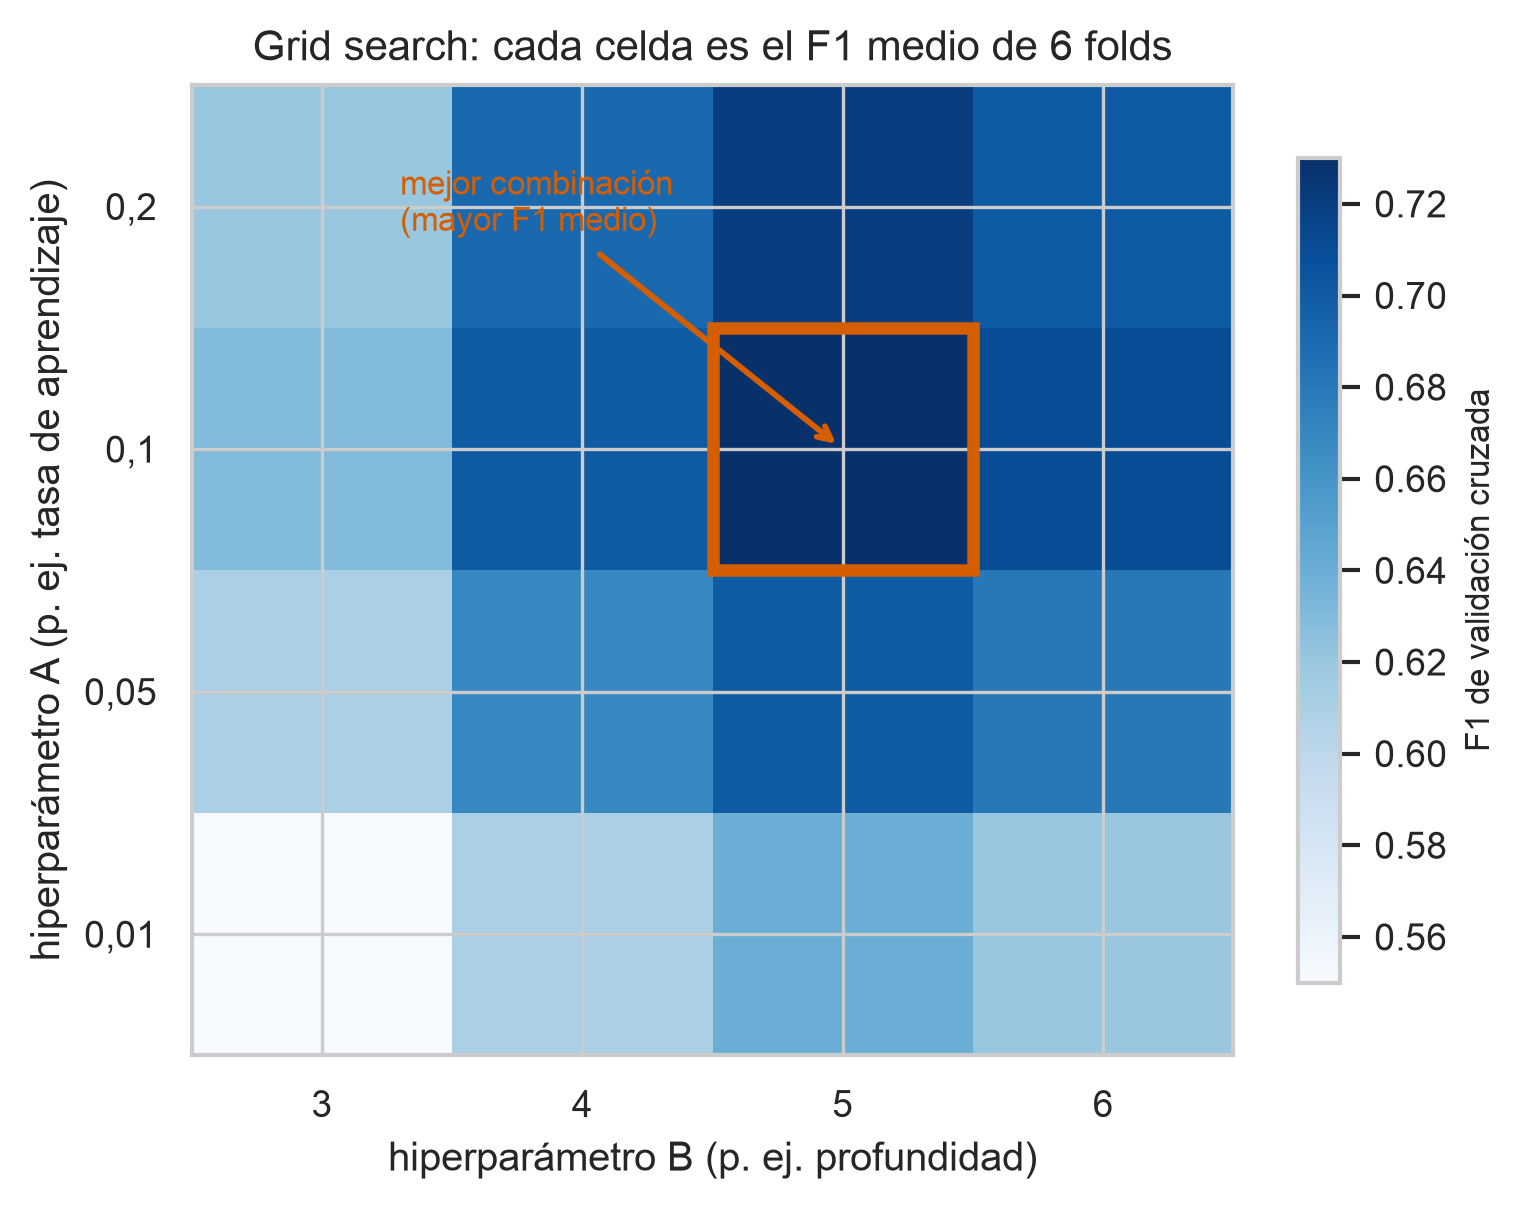
\includegraphics[width=0.5\textwidth]{concept_gridsearch}
\caption{Búsqueda en rejilla: cada celda es el rendimiento medio de una combinación de hiperparámetros
en validación cruzada; se conserva la mejor.}
\label{fig:gridsearch}
\end{figure}

\medskip
Fijado el protocolo, quedan los modelos empleados. Los presentamos en orden de complejidad creciente:
la regresión logística como referencia lineal, los vecinos más cercanos y la familia de los árboles de
decisión, sobre la que se construyen el bosque aleatorio y el gradient boosting.

\bigskip
\noindent\textbf{\large Regresión logística}
\label{sec:logreg}

\medskip
La regresión logística \cite{cox1958logreg} es el clasificador lineal por excelencia y sirve de
\textbf{modelo base}: la referencia simple e interpretable contra la que se miden los demás. La idea es modelar la probabilidad de la clase
positiva como una combinación lineal de las características, pero acotada al intervalo $(0,1)$ para que
pueda leerse como probabilidad. El acotado se hace mediante la función \emph{sigmoide}:
\begin{equation}
\sigma(z)=\frac{1}{1+e^{-z}},\qquad z = \beta_0 + \beta^{\top}x,\qquad p(y=1\mid x)=\sigma(z).
\label{eq:sigmoide}
\end{equation}
Aquí $\beta_0\in\mathbb{R}$ es el término independiente y $\beta\in\mathbb{R}^d$ el vector de
coeficientes, uno por característica. La sigmoide (Figura~\ref{fig:sigmoide}) comprime cualquier valor
real a $(0,1)$: valores muy negativos de $z$ dan probabilidad cercana a $0$, muy positivos cercana a
$1$, y $z=0$ da exactamente $0{,}5$, que marca la frontera de decisión.

\begin{figure}[H]
\centering
\begin{tikzpicture}[scale=0.95]
\draw[->] (-3.4,0)--(3.4,0) node[right]{$z$};
\draw[->] (0,-0.15)--(0,1.5) node[above]{$\sigma(z)$};
\draw[dashed] (-3.4,1)--(3.2,1) node[right]{$1$};
\draw[dashed] (-3.4,0.5)--(0,0.5) node[left]{$0{,}5$};
\draw[very thick,blue] plot[domain=-3.3:3.3,samples=100] (\x,{1/(1+exp(-2.2*\x))});
\filldraw[blue] (0,0.5) circle (1.4pt);
\end{tikzpicture}
\caption{Función sigmoide: transforma la combinación lineal $z$ en una probabilidad entre $0$ y $1$.}
\label{fig:sigmoide}
\end{figure}

La sigmoide admite una lectura muy útil si se despeja. Partiendo de $p=\sigma(z)=1/(1+e^{-z})$ se tiene
$1-p = e^{-z}/(1+e^{-z})$, y dividiendo,
\begin{equation}
\frac{p}{1-p} = e^{z}\quad\Longrightarrow\quad \log\frac{p}{1-p} = z = \beta_0 + \beta^{\top}x.
\label{eq:logodds}
\end{equation}
La combinación lineal es el logaritmo de la razón entre la probabilidad de la clase positiva y la de la
negativa, el \emph{log-odds}. Esta forma da a los coeficientes una lectura directa, y es la mayor
virtud del modelo: cada $\beta_i$ es cuánto varía el log-odds de la clase positiva al aumentar una
unidad la característica $i$, con las demás fijas. Su signo indica el sentido (un $\beta_i$ positivo
inclina la predicción hacia la clase positiva) y su magnitud, la fuerza.

Queda estimar los coeficientes $\beta$ a partir del entrenamiento. El criterio es la \textbf{máxima
verosimilitud}: elegir los $\beta$ que hacen más probables las etiquetas observadas. Con las
predicciones abreviadas $p_i=\sigma(\beta_0+\beta^{\top}x_i)$ y suponiendo los ejemplos independientes,
la verosimilitud de la base de datos es el producto de las probabilidades que el modelo asigna a cada
etiqueta real,
\begin{equation}
L(\beta) = \prod_{i=1}^{n} p_i^{\,y_i}\,(1-p_i)^{\,1-y_i},
\label{eq:verosim}
\end{equation}
donde el exponente selecciona el factor que toca: $p_i$ si $y_i=1$ y $1-p_i$ si $y_i=0$. Maximizar un
producto de muchos factores es poco práctico, por lo que se toman logaritmos, que convierten el producto en
suma y no alteran la posición del máximo, por ser el logaritmo creciente. Cambiando el signo para pasar de maximizar a
minimizar y dividiendo por $n$ para promediar, se obtiene la \emph{entropía cruzada}, la función de
pérdida que castiga predecir con confianza la clase equivocada:
\begin{equation}
\mathcal{L}(\beta) = -\frac{1}{n}\log L(\beta)
= -\frac{1}{n}\sum_{i=1}^{n}\Big[y_i\log p_i + (1-y_i)\log(1-p_i)\Big].
\label{eq:crossentropy}
\end{equation}
Cuando la etiqueta real es $y_i=1$, solo pesa el término $-\log p_i$, que crece sin cota cuando el
modelo asigna a ese ejemplo una probabilidad $p_i$ próxima a cero; cuando es $y_i=0$, pesa
$-\log(1-p_i)$, con el castigo simétrico. A diferencia de la regresión lineal, cuya pérdida cuadrática tiene la solución
cerrada $\hat\beta=(X^{\top}X)^{-1}X^{\top}y$, la entropía cruzada no se puede despejar: su gradiente
es no lineal en $\beta$. Sí es convexa, con lo que tiene un único mínimo, y ese mínimo se alcanza donde
el gradiente se anula. Usando la matriz de características $X\in\mathbb{R}^{n\times d}$, el vector de
etiquetas $y$ y el vector de predicciones $p=(p_1,\dots,p_n)^{\top}$, el gradiente tiene una forma
compacta,
\begin{equation}
\nabla_{\beta}\,\mathcal{L}(\beta) = \frac{1}{n}\,X^{\top}(p - y),
\label{eq:gradiente}
\end{equation}
el promedio de los errores $p_i-y_i$ ponderado por las características. Como no se anula en forma
cerrada, se resuelve por \textbf{descenso de gradiente}~\cite{cauchy1847gradient}: se parte de unos
coeficientes cualesquiera y se corrigen paso a paso en la dirección contraria al gradiente,
$\beta \leftarrow \beta - \eta\,\nabla_{\beta}\mathcal{L}$, con $\eta>0$ el tamaño de paso, hasta
converger. Es el mismo método que está en la base de muchos algoritmos de aprendizaje. Para frenar el
sobreajuste se añade un término de \textbf{regularización} que penaliza coeficientes grandes: la
penalización L2 los encoge de forma suave, y la L1 lleva algunos a cero exacto, con lo que además
descarta variables.

\begin{itemize}
\item \textbf{Ventajas:} interpretable por sus coeficientes, muy barata de entrenar y con
probabilidades bien calibradas.
\item \textbf{Desventajas:} solo traza fronteras lineales, por lo que resulta insuficiente cuando la
separación entre clases es curva; conviene además eliminar antes las variables muy correlacionadas
entre sí.
\end{itemize}

\bigskip
\noindent\textbf{\large K vecinos más cercanos}
\label{sec:knn}

\medskip
El clasificador de $k$ vecinos más cercanos (KNN) \cite{cover1967knn} no construye ningún modelo
explícito: guarda los datos de entrenamiento y clasifica cada ejemplo nuevo por \textbf{vecindad},
según la clase de los ejemplos más próximos. La idea plantea dos preguntas: dónde se sitúan
los datos y cómo se mide la cercanía. Lo primero se resuelve con el vector de características, que ubica
cada ejemplo como un punto de $\mathbb{R}^d$. Para lo segundo se usa una distancia; las más habituales
son la euclídea (la del teorema de Pitágoras) y la de Manhattan (la suma de diferencias en valor
absoluto, como recorrer una cuadrícula de calles),
\begin{equation}
d_{\text{euclídea}}(p,q)=\sqrt{\textstyle\sum_{i=1}^{d} (p_i-q_i)^2},\qquad
d_{\text{Manhattan}}(p,q)=\textstyle\sum_{i=1}^{d} |p_i-q_i|.
\label{eq:distancias}
\end{equation}
Ambas son casos de la distancia de Minkowski $\big(\sum_i |p_i-q_i|^r\big)^{1/r}$, con $r=2$ y $r=1$
respectivamente. Para clasificar un
punto nuevo se calculan sus distancias a todos los ejemplos de entrenamiento, se toman los $k$ más
cercanos y se le asigna la clase mayoritaria entre ellos (Figura~\ref{fig:knn}). La elección de $k$
cambia el resultado: en la figura, entre los tres vecinos más próximos gana una clase por dos votos a
uno, así que con $k=3$ el punto se clasifica en ella; al ampliar el radio a $k=5$ entran vecinos más
lejanos de la otra clase que pueden invertir el voto. El valor de $k$ es, por tanto, un hiperparámetro
que hay que fijar con cuidado.

\begin{figure}[H]
\centering
\begin{tikzpicture}[scale=1.05]
\filldraw[blue] (0.4,0.5) circle(2.5pt); \filldraw[blue] (0.9,1.1) circle(2.5pt);
\filldraw[blue] (0.3,1.4) circle(2.5pt); \filldraw[blue] (1.2,0.6) circle(2.5pt);
\filldraw[blue] (1.5,1.5) circle(2.5pt);
\draw[red,thick] (2.6,1.9) circle(2.5pt); \draw[red,thick] (3.0,1.4) circle(2.5pt);
\draw[red,thick] (2.3,2.3) circle(2.5pt); \draw[red,thick] (3.2,2.1) circle(2.5pt);
\draw[red,thick] (2.0,1.6) circle(2.5pt);
\filldraw[black] (1.9,1.5) circle(2.5pt) node[below=2pt,font=\footnotesize]{nuevo};
\draw[dashed] (1.9,1.5) circle(0.75) node[right=20pt,font=\footnotesize]{$k=3$};
\draw[dotted] (1.9,1.5) circle(1.25);
\end{tikzpicture}
\caption{KNN: el punto nuevo (negro) se clasifica por la clase mayoritaria entre sus vecinos. El
círculo interior es $k=3$; ampliar el radio ($k=5$) puede cambiar la decisión.}
\label{fig:knn}
\end{figure}

El parámetro $k$ gobierna el compromiso sesgo--varianza. Un $k$ pequeño hace la frontera muy sensible
al ruido local: con $k=1$ cada punto determina por sí solo su vecindad inmediata y basta un ejemplo mal
etiquetado para crear una región aislada de clase equivocada, lo que sobreajusta. Un $k$ grande promedia sobre
vecinos cada vez más lejanos, suaviza la frontera y aumenta el sesgo, hasta el extremo de que con $k=N$
todo punto recibe la clase mayoritaria global. El mejor valor depende de los datos y se busca por
validación, aunque una regla común de partida es $k=\sqrt{N}$, con $N$ el número de ejemplos. Como todo
se reduce a distancias, KNN es sensible a la escala de las variables y exige estandarizarlas antes. Sin
ese paso, una característica medida en miles (por ejemplo, la longitud de la respuesta en caracteres)
dominaría la distancia y anularía la contribución de otra acotada entre $0$ y $1$ (un solape), que
apenas influiría por pequeña que fuese su diferencia; estandarizar deja a todas en el mismo rango y con
el mismo peso a priori.

\begin{itemize}
\item \textbf{Ventajas:} no asume ninguna forma para la frontera entre clases, funciona bien con muchos
datos y no requiere una fase de entrenamiento.
\item \textbf{Desventajas:} clasificar es costoso, pues mide la distancia del punto nuevo a todo el
entrenamiento, y el método se degrada cuando hay muchas dimensiones o la distancia está mal elegida.
\end{itemize}

\bigskip
\noindent\textbf{\large Árboles de decisión}
\label{sec:arboles}

\medskip
Un árbol de decisión \cite{breiman1984cart,quinlan1986id3} clasifica imitando la forma en que una
persona decide mediante preguntas encadenadas, cada una más fina que la anterior, y es además la pieza
sobre la que se construyen los dos modelos siguientes. Tiene dos elementos: los \emph{nodos} internos,
donde se toma una decisión partiendo los datos por un umbral sobre una característica (``¿$x_1<u_1$?''),
y las \emph{hojas}, que asignan una clase (Figura~\ref{fig:arbol}). Clasificar un ejemplo
consiste en recorrer el árbol desde la raíz, respondiendo en cada nodo la pregunta con los valores de
ese ejemplo y siguiendo la rama correspondiente, hasta caer en una hoja, que da la clase predicha.

\begin{figure}[H]
\centering
\begin{tikzpicture}[
  every node/.style={font=\small},
  nodo/.style={rectangle, rounded corners, draw, align=center, inner sep=4pt},
  hoja/.style={rectangle, draw, fill=gray!12, align=center, inner sep=4pt},
  level 1/.style={sibling distance=46mm, level distance=13mm},
  level 2/.style={sibling distance=28mm, level distance=13mm}]
\node[nodo]{$x_1 < u_1$?}
  child{node[nodo]{$x_2 < u_2$?}
    child{node[hoja]{clase $1$} edge from parent node[left,font=\footnotesize]{sí}}
    child{node[hoja]{clase $0$} edge from parent node[right,font=\footnotesize]{no}}
    edge from parent node[left,font=\footnotesize]{sí}}
  child{node[hoja]{clase $0$} edge from parent node[right,font=\footnotesize]{no}};
\end{tikzpicture}
\caption{Árbol de decisión: los nodos parten los datos por un umbral; las hojas asignan la clase.}
\label{fig:arbol}
\end{figure}

El árbol se construye de arriba abajo. Se parte de la raíz, que contiene todos los ejemplos, y se
elige el corte que mejor separa las clases. Cada uno de los dos grupos resultantes se convierte en un
nodo nuevo al que se aplica el mismo procedimiento, y este se repite de forma recursiva sobre los
grupos que va generando hasta que dividir más no aporta mejora.

La pregunta en cada nodo es qué corte elegir de entre todos los posibles, uno por cada característica y
cada umbral sobre ella. El criterio es la \emph{pureza}: un buen corte deja a cada lado ejemplos de una
sola clase. La razón es que una hoja predice la clase mayoritaria de los
ejemplos que contiene, de modo que un grupo homogéneo se etiqueta sin error, mientras que uno donde las
clases se reparten a partes iguales no permite una predicción fiable.

La  \emph{impureza} mide cuánto se mezclan las clases en un nodo. Las dos más usadas son el índice de Gini y la entropía.

\begin{definicion}[Impureza de un nodo]
Sea un nodo con proporciones de clase $p_1,\dots,p_c$ (con $\sum_k p_k = 1$). Su \emph{índice de Gini}
y su \emph{entropía}~\cite{shannon1948entropy} son
\[
G = 1 - \sum_{k=1}^{c} p_k^2,\qquad H = -\sum_{k=1}^{c} p_k \log_2 p_k.
\]
Ambas valen cero cuando el nodo es puro (una sola clase, alguna $p_k=1$) y son máximas cuando las
clases están repartidas por igual.
\end{definicion}

\noindent Las dos cuantifican la mezcla de clases, pero con lecturas distintas. El índice de Gini es la
probabilidad de clasificar mal un ejemplo si se le asignara una clase al azar según las proporciones
del nodo; la entropía mide la incertidumbre del nodo. En un problema de dos clases, ambas son
máximas en el reparto mitad y mitad, donde el índice de Gini vale $0{,}5$ y la entropía, $1$.

La calidad de un corte se mide por cuánto baja la impureza al pasar del nodo padre a sus dos hijos. Si
el padre tiene impureza $I(\text{padre})$ y el corte lo divide en un hijo izquierdo y uno derecho, que
reciben una fracción $w_{\text{izq}}$ y $w_{\text{der}}$ de los ejemplos, la \emph{reducción de
impureza} del corte es
\begin{equation}
\Delta I = I(\text{padre})
         - \big(w_{\text{izq}}\,I(\text{izq}) + w_{\text{der}}\,I(\text{der})\big),
\label{eq:ganancia}
\end{equation}
esto es, la impureza del padre menos la impureza media de los hijos, en la que cada hijo pesa según la
fracción de ejemplos que recibe. El árbol elige en cada nodo el corte que hace máxima esa reducción.

Lo ilustramos con un ejemplo. Un nodo con $40$ ejemplos que alucinan y $60$ limpios tiene proporciones $0{,}4$
y $0{,}6$, luego su índice de Gini es
\[
G(\text{padre}) = 1 - 0{,}4^2 - 0{,}6^2 = 0{,}48.
\]
Consideremos un corte que lo divide en un hijo izquierdo con $30$ que alucinan y $10$ limpias, y un hijo
derecho con $10$ que alucinan y $50$ limpias. Cada hijo es más puro que el padre:
\[
G(\text{izq}) = 0{,}375, \qquad G(\text{der}) \approx 0{,}28.
\]
El hijo izquierdo recibe $40$ de los $100$ ejemplos y el derecho los $60$ restantes, así que la impureza
media de los hijos es
\[
\tfrac{40}{100}\cdot 0{,}375 + \tfrac{60}{100}\cdot 0{,}28 \approx 0{,}32,
\]
y la reducción que aporta el corte es $\Delta G = 0{,}48 - 0{,}32 \approx 0{,}16$. El árbol compara
así todos los cortes posibles y selecciona el de mayor reducción.

El procedimiento se repite en cada nodo nuevo y se detiene cuando el nodo ya es puro, cuando ningún
corte mejora la pureza o cuando se alcanza un límite fijado de antemano, como la profundidad máxima.

Sin restricciones, el árbol crece hasta separar por completo el entrenamiento y lo memoriza, lo que lo
hace muy flexible pero propenso al sobreajuste: un árbol profundo aprende las particularidades de los
datos y falla con datos nuevos. La profundidad máxima y el número mínimo de ejemplos por hoja son los
hiperparámetros que controlan ese crecimiento.

\begin{itemize}
\item \textbf{Ventajas:} captura interacciones entre variables, es insensible a la escala, maneja bien
características irrelevantes y su lógica es legible como una cadena de reglas.
\item \textbf{Desventajas:} un árbol único es inestable, pues pequeños cambios en los datos dan árboles
muy distintos, y sobreajusta con facilidad. Los dos modelos siguientes corrigen esto combinando muchos
árboles.
\end{itemize}

\bigskip
\noindent\textbf{\large Random Forest}
\label{sec:rf}

\medskip
El bosque aleatorio (\emph{Random Forest}) \cite{breiman2001rf} combina muchos árboles para ganar la
estabilidad de la que carece uno solo. Se apoya en una técnica llamada \emph{bagging} (\emph{bootstrap
aggregating}): de la base de entrenamiento se extraen $B$ muestras aleatorias con reemplazo, cada una
del mismo tamaño que la original pero con ejemplos repetidos y otros ausentes, y con cada muestra se
entrena un árbol distinto. Para clasificar un ejemplo nuevo, cada uno de los $B$ árboles emite su voto
y se toma la clase más votada,
\begin{equation}
\hat{y}(x) = \text{clase más votada entre } \{T_1(x),\dots,T_B(x)\}.
\label{eq:voto}
\end{equation}

El bagging reduce la varianza sin aumentar el sesgo. Para ver por qué, consideramos la versión con
predicciones numéricas, donde cada árbol devuelve la probabilidad de la clase positiva y el conjunto
las promedia. Si cada árbol individual tiene varianza
$\sigma^2$ y dos árboles distintos tienen una correlación $\rho$ entre sus predicciones, la varianza
del promedio de los $B$ árboles es
\begin{equation}
\mathrm{Var}\!\left(\frac{1}{B}\sum_{b=1}^{B} T_b(x)\right)
= \rho\,\sigma^2 + \frac{1-\rho}{B}\,\sigma^2.
\label{eq:varbagging}
\end{equation}
El segundo sumando se desvanece al crecer $B$, así que promediar muchos árboles cancela la parte no
correlacionada del ruido. El
primer sumando, en cambio, no depende de $B$: queda un suelo de varianza $\rho\,\sigma^2$ que solo baja
si los árboles están poco correlacionados. Como el promedio no cambia la predicción esperada, el sesgo
se mantiene. De aquí se sigue la estrategia del bosque: para reducir ese suelo de varianza hay que
descorrelacionar los árboles. El bagging ya los diferencia al entrenar cada uno con una muestra distinta, y el bosque añade
una segunda fuente de aleatoriedad: en cada corte no considera todas las características, sino un
subconjunto aleatorio de ellas (típicamente $\sqrt{d}$ de las $d$ disponibles en clasificación). Así ningún árbol
se apoya siempre en la misma variable dominante, baja $\rho$ y el conjunto gana estabilidad. El número
de árboles $B$, su profundidad y cuántas características se consideran en cada corte son sus
hiperparámetros, y suelen ajustarse por búsqueda.

\begin{itemize}
\item \textbf{Ventajas:} robusto y preciso, uno de los mejores clasificadores para datos tabulares;
hereda del árbol la captura de interacciones y la insensibilidad a la escala, maneja muchas variables y
apenas sobreajusta.
\item \textbf{Desventajas:} pierde la interpretabilidad de un árbol único, es más costoso de entrenar y
evaluar, y puede desajustarse con datos muy ruidosos si no se controla el número de árboles.
\end{itemize}

\bigskip
\noindent\textbf{\large Gradient boosting}
\label{sec:gb}

\medskip
El \emph{gradient boosting} \cite{friedman2001gbm} también combina árboles, pero de forma
\textbf{secuencial} en vez de paralela. En lugar de promediar árboles independientes que votan a la
vez, construye el modelo por etapas, de manera que cada árbol nuevo corrige los errores acumulados por los
anteriores. Empieza con una predicción sencilla y, en cada etapa, añade un árbol ajustado para reducir
ese error residual.

La clave del método es qué error corrige cada árbol nuevo. Tras $m-1$ etapas el modelo $F_{m-1}$ deja
en cada ejemplo un \emph{residuo}, la diferencia entre la etiqueta real y lo que predice. El \emph{boosting}
entrena el árbol siguiente para predecir ese residuo, de modo que sumarlo al modelo acerca la
predicción a la etiqueta. En su forma general, el residuo que se corrige es el gradiente de la función
de pérdida evaluado en las predicciones actuales, de ahí el nombre del método: cada árbol da un paso de
descenso de gradiente, pero en el espacio de las funciones en vez de en el de unos coeficientes. El
modelo tras $m$ etapas es el anterior más el árbol nuevo,
\begin{equation}
F_m(x) = F_{m-1}(x) + \nu\, h_m(x),
\label{eq:boosting}
\end{equation}
donde $h_m$ es el árbol de la etapa $m$, ajustado a los gradientes que deja $F_{m-1}$, y $\nu\in(0,1]$
es la \textbf{tasa de aprendizaje} o \emph{shrinkage}, que modera cuánto contribuye cada árbol.
Reducir cada paso frena la corrección: una tasa pequeña avanza despacio y necesita más árboles, pero
generaliza mejor, porque ningún árbol individual domina el resultado; una tasa grande, o demasiados
árboles, sobreajustan. Tasa de aprendizaje y número de árboles se ajustan juntos, por ser las dos caras
del mismo compromiso. A esa \textbf{regularización} por \emph{shrinkage} se suman otras: limitar la
profundidad de cada árbol para que corrija tendencias generales y no casos aislados, entrenar cada árbol
sobre una submuestra aleatoria de los datos, y penalizar la complejidad del árbol en la propia función
de pérdida.

La diferencia con el bosque aleatorio es de fondo. El bosque promedia árboles independientes para
reducir la \emph{varianza}, partiendo de árboles que ya de por sí aciertan; el boosting encadena
árboles dependientes, cada uno corrigiendo lo que el anterior no logró, para reducir el \emph{sesgo},
partiendo de un modelo débil que va mejorando. Eso suele dar mayor precisión, a cambio de un ajuste más
delicado y más lento. \textbf{XGBoost} \cite{chen2016xgboost} es una implementación eficiente y
regularizada de esta idea, referencia habitual en problemas sobre datos tabulares.

\begin{itemize}
\item \textbf{Ventajas:} suele ofrecer la mayor precisión de los modelos clásicos sobre datos
tabulares y maneja bien las interacciones entre variables.
\item \textbf{Desventajas:} tiene más hiperparámetros que ajustar, entrena más despacio que un bosque y
su riesgo de sobreajuste es mayor si no se regula con cuidado.
\end{itemize}

\subsection{Valoración}

La \textbf{valoración} cuantifica el rendimiento de los modelos ajustados sobre datos no empleados en el
entrenamiento. Una \emph{métrica} es un indicador de la calidad del modelo; todas las empleadas se
construyen sobre el mismo recuento de aciertos y errores.

Tomando como clase positiva la que interesa detectar (la alucinación), cada predicción pertenece a una
de estas cuatro categorías:

\begin{itemize}
\item \textbf{Verdaderos positivos (VP):} alucinaciones que el modelo marca como alucinación (acierto).
\item \textbf{Verdaderos negativos (VN):} respuestas limpias que marca como limpias (acierto).
\item \textbf{Falsos positivos (FP):} respuestas limpias que marca como alucinación (error de tipo I,
una falsa alarma).
\item \textbf{Falsos negativos (FN):} alucinaciones que marca como limpias (error de tipo II, una
invención que pasa inadvertida).
\end{itemize}

Estos cuatro conteos se organizan en la \emph{matriz de confusión} (Cuadro~\ref{tab:confusion}), que
cruza la clase real de cada respuesta con la predicha por el modelo.

\begin{table}[H]
\centering
\renewcommand{\arraystretch}{1.3}
\setlength{\tabcolsep}{9pt}
\begin{tabular}{|c|c|c|c|}
\hline
\multicolumn{2}{|c|}{\multirow{2}{*}{}} & \multicolumn{2}{c|}{\textbf{Predicción del modelo}} \\
\cline{3-4}
\multicolumn{2}{|c|}{} & \textbf{Alucinación} & \textbf{Limpia} \\
\hline
\multirow{2}{*}{\rotatebox{90}{\textbf{Clase real}\,}} & \textbf{Alucinación}
  & \makecell{\textbf{VP} \\ verdadero positivo \\ (acierto)}
  & \makecell{\textbf{FN} \\ falso negativo \\ (error de tipo II)} \\
\cline{2-4}
 & \textbf{Limpia}
  & \makecell{\textbf{FP} \\ falso positivo \\ (error de tipo I)}
  & \makecell{\textbf{VN} \\ verdadero negativo \\ (acierto)} \\
\hline
\end{tabular}
\caption{Matriz de confusión. Cada respuesta cae en una de las cuatro casillas según su clase real
(filas) y la predicción del modelo (columnas). Los aciertos ($VP$ y $VN$) quedan en la diagonal; el
falso negativo (error de tipo II) es una alucinación que pasa inadvertida y el falso positivo (error de
tipo I), una falsa alarma sobre una respuesta limpia.}
\label{tab:confusion}
\end{table}

Los dos errores rara vez cuestan lo mismo. En un diagnóstico médico, un falso negativo deja sin tratar
a un enfermo, mientras que un falso positivo trata a un sano. En la detección de alucinaciones el error
caro es el falso negativo, una invención que llega al usuario sin control.

\medskip
\noindent\textbf{Precisión.} De todas las respuestas que el modelo marca como alucinación, la fracción
que lo son realmente. Mide la fiabilidad del modelo al señalar una alucinación: un valor cercano a $1$
indica que casi nunca se equivoca cuando predice un positivo.
\begin{equation}
\mathrm{precisión} = \frac{VP}{VP+FP}.
\label{eq:precision}
\end{equation}

\medskip
\noindent\textbf{Cobertura} (también exhaustividad o sensibilidad)\textbf{.} De todas las alucinaciones
reales, la fracción que el modelo detecta. Un valor cercano a $1$ indica que detecta casi todas.
\begin{equation}
\mathrm{cobertura} = \frac{VP}{VP+FN}.
\label{eq:recall}
\end{equation}

\medskip
\noindent\textbf{Especificidad.} La cobertura de la clase negativa: de todas las respuestas limpias, la
fracción que el modelo reconoce como tales. Interviene en las métricas que equilibran ambas clases.
\begin{equation}
\mathrm{especificidad} = \frac{VN}{VN+FP}.
\label{eq:especificidad}
\end{equation}

\medskip
Precisión y cobertura varían en sentidos opuestos, y el umbral de decisión fija el equilibrio entre
ambas. Si el modelo solo predice positivo cuando tiene alta confianza, acierta casi siempre que lo hace
(precisión alta) pero omite los positivos dudosos (cobertura baja); si predice positivo con poca
evidencia, apenas omite ninguno (cobertura alta) a costa de numerosas falsas alarmas (precisión baja).
Las métricas siguientes resumen ese equilibrio en un solo número.

\medskip
\noindent\textbf{Valor $F_1$.} Combina precisión y cobertura en su \emph{media armónica}, que solo es alta
cuando ambas lo son; si una se acerca a cero, el valor de $F_1$ también.
\begin{equation}
F_1 = 2\,\frac{\mathrm{precisión}\cdot\mathrm{cobertura}}{\mathrm{precisión}+\mathrm{cobertura}}.
\label{eq:f1}
\end{equation}
Se prefiere la media armónica a la aritmética porque esta valdría $0{,}5$ para un modelo con precisión
$1$ y cobertura $0$, que no detecta nada.

\medskip
\noindent\textbf{Valor $F_\beta$.} El $F_1$ da igual peso a precisión y cobertura. Su generalización $F_\beta$ pondera la cobertura $\beta^2$ veces más que la precisión; el caso
$\beta=2$ ($F_2$) lo pesa cuatro veces más, útil cuando el falso negativo es el error caro.
\begin{equation}
F_\beta = (1+\beta^2)\,\frac{\mathrm{precisión}\cdot\mathrm{cobertura}}
{\beta^2\,\mathrm{precisión}+\mathrm{cobertura}}.
\label{eq:fbeta}
\end{equation}

\medskip
\noindent\textbf{Accuracy.} La fracción de aciertos sobre el total. Es intuitiva, pero resulta engañosa
cuando una clase domina: si el $90\,\%$ de los ejemplos son negativos, predecir siempre negativo ya da
un $90\,\%$ de accuracy sin detectar un solo positivo.
\begin{equation}
\mathrm{accuracy} = \frac{VP+VN}{VP+VN+FP+FN}.
\label{eq:accuracy}
\end{equation}

\medskip
\noindent\textbf{Balanced accuracy.} Corrige esa distorsión promediando la tasa de aciertos de cada
clase por separado: la cobertura en la clase positiva y la especificidad en la negativa. Así la clase
minoritaria pesa igual que la mayoritaria.
\begin{equation}
\mathrm{balanced\ accuracy} = \tfrac12\big(\mathrm{cobertura}+\mathrm{especificidad}\big).
\label{eq:balacc}
\end{equation}

\medskip
Un ejemplo numérico ilustra las definiciones anteriores. Sobre $300$ respuestas con $100$ alucinaciones
reales, un detector acierta $70$ ($VP=70$, $FN=30$) a costa de $20$ falsas alarmas ($FP=20$, $VN=180$).
Entonces
\[
\mathrm{precisión}=\frac{70}{90}\approx0{,}78,\quad
\mathrm{cobertura}=\frac{70}{100}=0{,}70,\quad
F_1\approx0{,}74,\quad
\mathrm{accuracy}=\frac{250}{300}\approx0{,}83.
\]
La accuracy ($0{,}83$) resulta alta porque el modelo acierta casi todos los negativos, que son mayoría;
la balanced accuracy, $\tfrac12(0{,}70+0{,}90)=0{,}80$, corrige esa cifra al dar el mismo peso a las dos
clases.

\medskip
Todas las métricas anteriores dependen del umbral con que la probabilidad se convierte en decisión. Dos
curvas recorren todos los umbrales a la vez.

\medskip
\noindent\textbf{Curva ROC y AUC.} La curva ROC contrapone la tasa de verdaderos positivos (la cobertura)
frente a la tasa de falsos positivos al variar el umbral \cite{fawcett2006roc}. Su área bajo la curva,
el \textbf{AUC}, resume en una sola cifra el rendimiento en todos los umbrales.

\begin{teorema}[Área bajo la curva ROC]
Sea $s(x)$ la puntuación que el clasificador asigna a un ejemplo $x$, y sean $X^{+}$ y $X^{-}$ un
positivo y un negativo tomados al azar de forma independiente. El área bajo la curva ROC coincide con
la probabilidad de que el positivo puntúe por encima del negativo:
\[
\mathrm{AUC} \;=\; \int_0^1 \mathrm{TVP}\big(\mathrm{TFP}\big)\,\mathrm{d}(\mathrm{TFP})
\;=\; \mathbb{P}\!\left(s(X^{+}) > s(X^{-})\right),
\]
con el convenio de contar como $\tfrac12$ los empates $s(X^{+})=s(X^{-})$.
\end{teorema}

\noindent La primera igualdad es la lectura geométrica; la segunda, la probabilística
\cite{hanley1982roc}. El AUC tiene dos propiedades que lo hacen sólido para comparar modelos:

\begin{itemize}
\item es invariante a la escala del score, pues solo importa el orden de las predicciones;
\item es invariante al umbral, pues los resume todos, así que compara sin fijar un punto de operación.
\end{itemize}

\medskip
\noindent\textbf{Curva precisión--cobertura.} Contrapone precisión frente a cobertura al variar el umbral. A
diferencia del AUC, sí refleja el desbalance, porque la precisión depende de la proporción de
positivos; por ello resulta más informativa que el AUC cuando la clase positiva es minoritaria. Un buen
modelo mantiene la precisión alta aun a cobertura alta, y su curva se acerca a la esquina superior
derecha.

\begin{figure}[H]
\centering
\begin{tikzpicture}[scale=1.9]
\draw[->] (0,0)--(1.12,0) node[right,font=\footnotesize]{tasa de FP};
\draw[->] (0,0)--(0,1.12) node[above,font=\footnotesize]{tasa de VP};
\draw[dashed] (0,0)--(1,1) node[pos=0.6,below right,font=\footnotesize]{azar};
\draw[very thick,blue] (0,0) .. controls (0.05,0.6) and (0.25,0.95) .. (1,1);
\node[font=\footnotesize] at (0.58,0.4) {AUC};
\node[font=\small] at (0.5,-0.28) {(a) curva ROC};
\begin{scope}[xshift=3.4cm]
\draw[->] (0,0)--(1.12,0) node[right,font=\footnotesize]{cobertura};
\draw[->] (0,0)--(0,1.12) node[above,font=\footnotesize]{precisión};
\draw[very thick,blue] (0,0.97) .. controls (0.6,0.95) and (0.8,0.85) .. (1,0.35);
\node[font=\small] at (0.5,-0.28) {(b) curva precisión--cobertura};
\end{scope}
\end{tikzpicture}
\caption{Las dos curvas que recorren todos los umbrales. La ROC resume la separación en el AUC; la
precisión--cobertura muestra a partir de qué cobertura se degrada la precisión.}
\label{fig:curvas}
\end{figure}

\medskip
\noindent\textbf{Índice de Youden.} Fijado el modelo, resta determinar el umbral que convierte su
\emph{score} en decisión. El índice de Youden selecciona el que maximiza
\begin{equation}
J = \mathrm{sensibilidad} + \mathrm{especificidad} - 1,
\label{eq:youden}
\end{equation}
esto es, el punto de la curva ROC más alejado de la diagonal, donde mejor se separan las dos clases
\cite{youden1950index}. Rebajar el umbral aumenta la cobertura a costa de la precisión, y elevarlo
produce el efecto contrario; el umbral es, por tanto, junto al remuestreo, una palanca frente al
desbalance.

\bibliographystyle{plain}
\bibliography{referencias}

\end{document}
